% Options for packages loaded elsewhere
\PassOptionsToPackage{unicode}{hyperref}
\PassOptionsToPackage{hyphens}{url}
%
\documentclass[
  man]{apa6}
\usepackage{amsmath,amssymb}
\usepackage{lmodern}
\usepackage{iftex}
\ifPDFTeX
  \usepackage[T1]{fontenc}
  \usepackage[utf8]{inputenc}
  \usepackage{textcomp} % provide euro and other symbols
\else % if luatex or xetex
  \usepackage{unicode-math}
  \defaultfontfeatures{Scale=MatchLowercase}
  \defaultfontfeatures[\rmfamily]{Ligatures=TeX,Scale=1}
\fi
% Use upquote if available, for straight quotes in verbatim environments
\IfFileExists{upquote.sty}{\usepackage{upquote}}{}
\IfFileExists{microtype.sty}{% use microtype if available
  \usepackage[]{microtype}
  \UseMicrotypeSet[protrusion]{basicmath} % disable protrusion for tt fonts
}{}
\makeatletter
\@ifundefined{KOMAClassName}{% if non-KOMA class
  \IfFileExists{parskip.sty}{%
    \usepackage{parskip}
  }{% else
    \setlength{\parindent}{0pt}
    \setlength{\parskip}{6pt plus 2pt minus 1pt}}
}{% if KOMA class
  \KOMAoptions{parskip=half}}
\makeatother
\usepackage{xcolor}
\usepackage{graphicx}
\makeatletter
\def\maxwidth{\ifdim\Gin@nat@width>\linewidth\linewidth\else\Gin@nat@width\fi}
\def\maxheight{\ifdim\Gin@nat@height>\textheight\textheight\else\Gin@nat@height\fi}
\makeatother
% Scale images if necessary, so that they will not overflow the page
% margins by default, and it is still possible to overwrite the defaults
% using explicit options in \includegraphics[width, height, ...]{}
\setkeys{Gin}{width=\maxwidth,height=\maxheight,keepaspectratio}
% Set default figure placement to htbp
\makeatletter
\def\fps@figure{htbp}
\makeatother
\setlength{\emergencystretch}{3em} % prevent overfull lines
\providecommand{\tightlist}{%
  \setlength{\itemsep}{0pt}\setlength{\parskip}{0pt}}
\setcounter{secnumdepth}{-\maxdimen} % remove section numbering
% Make \paragraph and \subparagraph free-standing
\ifx\paragraph\undefined\else
  \let\oldparagraph\paragraph
  \renewcommand{\paragraph}[1]{\oldparagraph{#1}\mbox{}}
\fi
\ifx\subparagraph\undefined\else
  \let\oldsubparagraph\subparagraph
  \renewcommand{\subparagraph}[1]{\oldsubparagraph{#1}\mbox{}}
\fi
\newlength{\cslhangindent}
\setlength{\cslhangindent}{1.5em}
\newlength{\csllabelwidth}
\setlength{\csllabelwidth}{3em}
\newlength{\cslentryspacingunit} % times entry-spacing
\setlength{\cslentryspacingunit}{\parskip}
\newenvironment{CSLReferences}[2] % #1 hanging-ident, #2 entry spacing
 {% don't indent paragraphs
  \setlength{\parindent}{0pt}
  % turn on hanging indent if param 1 is 1
  \ifodd #1
  \let\oldpar\par
  \def\par{\hangindent=\cslhangindent\oldpar}
  \fi
  % set entry spacing
  \setlength{\parskip}{#2\cslentryspacingunit}
 }%
 {}
\usepackage{calc}
\newcommand{\CSLBlock}[1]{#1\hfill\break}
\newcommand{\CSLLeftMargin}[1]{\parbox[t]{\csllabelwidth}{#1}}
\newcommand{\CSLRightInline}[1]{\parbox[t]{\linewidth - \csllabelwidth}{#1}\break}
\newcommand{\CSLIndent}[1]{\hspace{\cslhangindent}#1}
\ifLuaTeX
\usepackage[bidi=basic]{babel}
\else
\usepackage[bidi=default]{babel}
\fi
\babelprovide[main,import]{english}
% get rid of language-specific shorthands (see #6817):
\let\LanguageShortHands\languageshorthands
\def\languageshorthands#1{}
% Manuscript styling
\usepackage{upgreek}
\captionsetup{font=singlespacing,justification=justified}

% Table formatting
\usepackage{longtable}
\usepackage{lscape}
% \usepackage[counterclockwise]{rotating}   % Landscape page setup for large tables
\usepackage{multirow}		% Table styling
\usepackage{tabularx}		% Control Column width
\usepackage[flushleft]{threeparttable}	% Allows for three part tables with a specified notes section
\usepackage{threeparttablex}            % Lets threeparttable work with longtable

% Create new environments so endfloat can handle them
% \newenvironment{ltable}
%   {\begin{landscape}\centering\begin{threeparttable}}
%   {\end{threeparttable}\end{landscape}}
\newenvironment{lltable}{\begin{landscape}\centering\begin{ThreePartTable}}{\end{ThreePartTable}\end{landscape}}

% Enables adjusting longtable caption width to table width
% Solution found at http://golatex.de/longtable-mit-caption-so-breit-wie-die-tabelle-t15767.html
\makeatletter
\newcommand\LastLTentrywidth{1em}
\newlength\longtablewidth
\setlength{\longtablewidth}{1in}
\newcommand{\getlongtablewidth}{\begingroup \ifcsname LT@\roman{LT@tables}\endcsname \global\longtablewidth=0pt \renewcommand{\LT@entry}[2]{\global\advance\longtablewidth by ##2\relax\gdef\LastLTentrywidth{##2}}\@nameuse{LT@\roman{LT@tables}} \fi \endgroup}

% \setlength{\parindent}{0.5in}
% \setlength{\parskip}{0pt plus 0pt minus 0pt}

% Overwrite redefinition of paragraph and subparagraph by the default LaTeX template
% See https://github.com/crsh/papaja/issues/292
\makeatletter
\renewcommand{\paragraph}{\@startsection{paragraph}{4}{\parindent}%
  {0\baselineskip \@plus 0.2ex \@minus 0.2ex}%
  {-1em}%
  {\normalfont\normalsize\bfseries\itshape\typesectitle}}

\renewcommand{\subparagraph}[1]{\@startsection{subparagraph}{5}{1em}%
  {0\baselineskip \@plus 0.2ex \@minus 0.2ex}%
  {-\z@\relax}%
  {\normalfont\normalsize\itshape\hspace{\parindent}{#1}\textit{\addperi}}{\relax}}
\makeatother

% \usepackage{etoolbox}
\makeatletter
\patchcmd{\HyOrg@maketitle}
  {\section{\normalfont\normalsize\abstractname}}
  {\section*{\normalfont\normalsize\abstractname}}
  {}{\typeout{Failed to patch abstract.}}
\patchcmd{\HyOrg@maketitle}
  {\section{\protect\normalfont{\@title}}}
  {\section*{\protect\normalfont{\@title}}}
  {}{\typeout{Failed to patch title.}}
\makeatother

\usepackage{xpatch}
\makeatletter
\xapptocmd\appendix
  {\xapptocmd\section
    {\addcontentsline{toc}{section}{\appendixname\ifoneappendix\else~\theappendix\fi\\: #1}}
    {}{\InnerPatchFailed}%
  }
{}{\PatchFailed}
\keywords{\newline\indent Word count: X}
\DeclareDelayedFloatFlavor{ThreePartTable}{table}
\DeclareDelayedFloatFlavor{lltable}{table}
\DeclareDelayedFloatFlavor*{longtable}{table}
\makeatletter
\renewcommand{\efloat@iwrite}[1]{\immediate\expandafter\protected@write\csname efloat@post#1\endcsname{}}
\makeatother
\usepackage{lineno}

\linenumbers
\usepackage{csquotes}
\ifLuaTeX
  \usepackage{selnolig}  % disable illegal ligatures
\fi
\IfFileExists{bookmark.sty}{\usepackage{bookmark}}{\usepackage{hyperref}}
\IfFileExists{xurl.sty}{\usepackage{xurl}}{} % add URL line breaks if available
\urlstyle{same} % disable monospaced font for URLs
\hypersetup{
  pdftitle={Supplementary Materials for Perpecptual Salience of Positive Self},
  pdfauthor={Hu Chuan-Peng1,2, Kaiping Peng2, \& Jie Sui2,3},
  pdflang={en-EN},
  hidelinks,
  pdfcreator={LaTeX via pandoc}}

\title{Supplementary Materials for Perpecptual Salience of Positive Self}
\author{Hu Chuan-Peng\textsuperscript{1,2}, Kaiping Peng\textsuperscript{2}, \& Jie Sui\textsuperscript{2,3}}
\date{}


\shorttitle{Supplementary Materials}

\authornote{

Hu Chuan-Peng, School of Psychology, Nanjing Normal University, 210024 Nanjing, China.
Kaiping Peng, Department of Psychology, Tsinghua University, 100084 Beijing, China.
Jie Sui, School of Psychology, University of Aberdeen, Aberdeen, Scotland.
Authors contriubtion: HCP, JS, \& KP design the study, HCP collected the data, HCP analyzed the data and drafted the manuscript. All authors read and agreed upon the current version of the manuscripts.

Authors contriubtion: HCP, JS, \& KP design the study, HCP collected the data, HCP analyzed the data and drafted the manuscript. KP \& JS supported this project.

Correspondence concerning this article should be addressed to Hu Chuan-Peng, School of Psychology, Nanjing Normal University, Ninghai Road 122, Gulou District, 210024 Nanjing, China. E-mail: \href{mailto:hcp4715@hotmail.com}{\nolinkurl{hcp4715@hotmail.com}}

}

\affiliation{\vspace{0.5cm}\textsuperscript{1} Nanjing Normal University, 210024 Nanjing, China\\\textsuperscript{2} Tsinghua University, 100084 Beijing, China\\\textsuperscript{3} University of Aberdeen, Aberdeen, Scotland}

\begin{document}
\maketitle

\hypertarget{about-the-supplementary}{%
\section{About the Supplementary}\label{about-the-supplementary}}

Here we described the details of each experiment, without the results. For demonstrating purpose, we plot the results for each experiment. As the de-identified raw data are open, interested readers can easily get the results without much difficult.

\hypertarget{experiment-1a}{%
\section{Experiment 1a}\label{experiment-1a}}

\hypertarget{methods}{%
\subsection{Methods}\label{methods}}

\hypertarget{participants}{%
\subsubsection{Participants}\label{participants}}

57 college students (38 female, age = 20.75 \(\pm\) 2.54 years) participated. 39 of them were recruited from Tsinghua University community in 2014; 18 were recruited from Wenzhou University in 2017. All participants were right-handed except one, and all had normal or corrected-to-normal vision. Informed consent was obtained from all participants prior to the experiment according to procedures approved by the local ethics committees. 6 participant's data were excluded from analysis because nearly random level of accuracy, leaving 51 participants (34 female, age = 20.72 \(\pm\) 2.44 years).

\hypertarget{stimuli-and-tasks}{%
\subsubsection{Stimuli and Tasks}\label{stimuli-and-tasks}}

Three geometric shapes were used in this experiment: triangle, square, and circle. These shapes were paired with three labels (bad person, good person or neutral person). The pairs were counterbalanced across participants.

\hypertarget{procedure}{%
\subsubsection{Procedure}\label{procedure}}

As we describe in general method part, this experiment had two phases. First, there was a learning stage. Participants were asked to learn the relationship between geometric shapes (triangle, square, and circle) and different person (bad person, a good person, or a neutral person). For example, a participant was told, ``bad person is a circle; good person is a triangle; and a neutral person is represented by a square.'' After participant remember the associations (usually in a few minutes), participants started a practicing phase of matching task which has the exact task as in the experimental task.
In the experimental task, participants judged whether shape--label pairs, which were subsequently presented, were correct. Each trial started with the presentation of a central fixation cross for 500 ms. Subsequently, a pairing of a shape and label (good person, bad person, and neutral person) was presented for 100 ms. The pair presented could confirm to the verbal instruction for each pairing given in the training stage, or it could be a recombination of a shape with a different label, with the shape--label pairings being generated at random. The next frame showed a blank for 1100ms. Participants were expected to judge whether the shape was correctly assigned to the person by pressing one of the two response buttons as quickly and accurately as possible within this timeframe (to encourage immediate responding). Feedback (correct or incorrect) was given on the screen for 500 ms at the end of each trial, if no response detected, ``too slow'' was presented to remind participants to accelerate. Participants were informed of their overall accuracy at the end of each block. The practice phase finished and the experimental task began after the overall performance of accuracy during practice phase achieved 60\%.
For participants from the Tsinghua community, they completed 6 experimental blocks of 60 trials. Thus, there were 60 trials in each condition (bad-person match, bad-person nonmatch, good-person match, good-person nonmatch, neutral-person match, and neutral-person nonmatch). For the participants from Wenzhou University, they finished 6 blocks of 120 trials, therefore, 120 trials for each condition.

\hypertarget{descriptive-results}{%
\subsection{Descriptive results}\label{descriptive-results}}

\begin{figure}
\centering
\includegraphics{Suppl_Materials_individual_Exp_simple_files/figure-latex/exp1a-dprime-rt-1.pdf}
\caption{\label{fig:exp1a-dprime-rt}RT and \emph{d} prime of Experiment 1a.}
\end{figure}

\hypertarget{experiment-1b}{%
\section{Experiment 1b}\label{experiment-1b}}

In this study, we aimed at excluding the potential confounding factor of the familiarity of words we used in experiment 1a, by matching the familiarity of the words.

\hypertarget{method}{%
\subsection{Method}\label{method}}

\hypertarget{participants-1}{%
\subsubsection{Participants}\label{participants-1}}

72 college students (49 female, age = 20.17 \(\pm\) 2.08 years) participated. 39 of them were recruited from Tsinghua University community in 2014; 33 were recruited from Wenzhou University in 2017. All participants were right-handed except one, and all had normal or corrected-to-normal vision. Informed consent was obtained from all participants prior to the experiment according to procedures approved by the local ethics committees. 20 participant's data were excluded from analysis because nearly random level of accuracy, leaving 52 participants (36 female, age = 20.25 \(\pm\) 2.31 years).

\hypertarget{stimuli-and-tasks-1}{%
\subsubsection{Stimuli and Tasks}\label{stimuli-and-tasks-1}}

Three geometric shapes (triangle, square, and circle, with 3.7º × 3.7º of visual angle) were presented above a white fixation cross subtending 0.8º × 0.8º of visual angle at the center of the screen. The three shapes were randomly assigned to three labels with different moral valence: a morally bad person (``恶人'', ERen), a morally good person (``善人'', ShanRen) or a morally neutral person (``常人'', ChangRen). The order of the associations between shapes and labels was counterbalanced across participants.
Three labels used in this experiment is selected based on the rating results from an independent survey, in which participants rated the familiarity, frequency, and concreteness of eight different words online. Of the eight words, three of them are morally positive (HaoRen, ShanRen, Junzi), two of them are morally neutral (ChangRen, FanRen), and three of them are morally negative (HuaiRen, ERen, LiuMang). An independent sample consist of 35 participants (22 females, age 20.6 ± 3.11) were recruited to rate these words. Based on the ratings (see supplementary materials Figure S1), we selected ShanRen, ChangRen, and ERen to represent morally positive, neutral, and negative person.
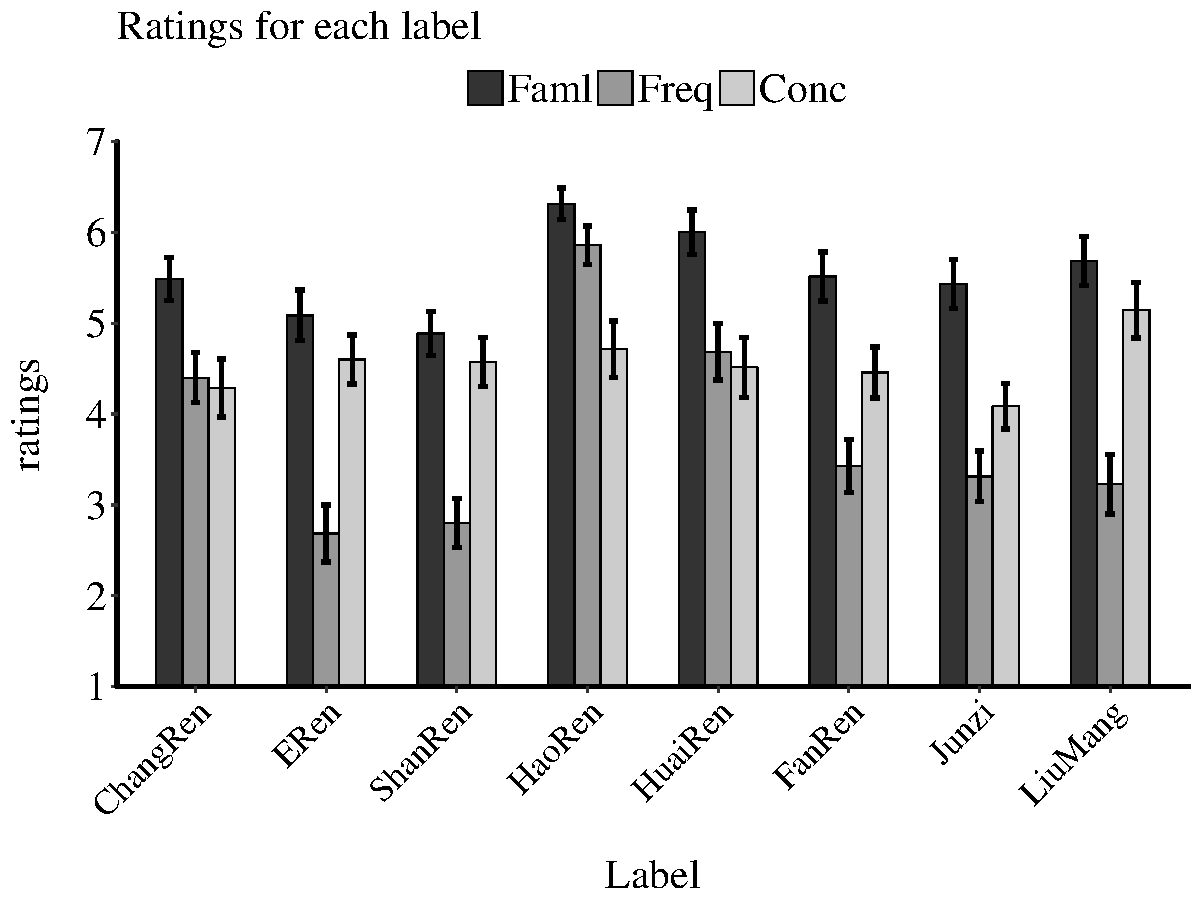
\includegraphics[width=5.20833in,height=\textheight]{exp1b/Familiarity_ratings/df1b_fami_rating.pdf}

\hypertarget{procedure-1}{%
\subsubsection{Procedure}\label{procedure-1}}

For participants from both Tsinghua community and Wenzhou community, the procedure in the current study was exactly same as in experiment 1a.

\hypertarget{descriptive-results-1}{%
\subsection{Descriptive results}\label{descriptive-results-1}}

\begin{figure}
\centering
\includegraphics{Suppl_Materials_individual_Exp_simple_files/figure-latex/exp1b-dprime-rt-1.pdf}
\caption{\label{fig:exp1b-dprime-rt}RT and \emph{d} prime of Experiment 1b.}
\end{figure}

\hypertarget{experiment-1c}{%
\section{Experiment 1c}\label{experiment-1c}}

In this study, we further control the valence of words using in our experiment. Instead of using label with moral valence, we used valence-neutral names in China. Participant first learn behaviors of the different person, then, they associate the names and shapes. And then they perform a name-shape matching task.

\hypertarget{method-1}{%
\subsection{Method}\label{method-1}}

\hypertarget{participants-2}{%
\subsubsection{Participants}\label{participants-2}}

23 college students (15 female, age = 22.61 \(\pm\) 2.62 years) participated. All of them were recruited from Tsinghua University community in 2014. Informed consent was obtained from all participants prior to the experiment according to procedures approved by the local ethics committees. No participant was excluded because they overall accuracy were above 0.6.

\hypertarget{stimuli-and-tasks-2}{%
\subsubsection{Stimuli and Tasks}\label{stimuli-and-tasks-2}}

Three geometric shapes (triangle, square, and circle, with 3.7º × 3.7º of visual angle) were presented above a white fixation cross subtending 0.8º × 0.8º of visual angle at the center of the screen. The three most common names were chosen, which are neutral in moral valence before the manipulation.
Three names (Zhang, Wang, Li) were first paired with three paragraphs of behavioral description. Each description includes one sentence of biographic information and four sentences that describing the moral behavioral under that name. To assess the that these three descriptions represented good, neutral, and bad valence, we collected the ratings of three person on six dimensions: morality, likability, trustworthiness, dominance, competence, and aggressiviess, from an independent sample (n = 34, 18 female, age = 19.6 ± 2.05). The rating results showed that the person with morally good behavioral description has higher score on morality (M = 3.59, SD = 0.66) than neutral (M = 0.88, SD = 1.1), \emph{t}(33) = 12.94, \emph{p} \textless{} .001, and bad conditions (M = -3.4, SD = 1.1), \emph{t}(33) = 30.78, \emph{p} \textless{} .001. Neutral condition was also significant higher than bad conditions \(t(33) = 13.9\), \(p < .001\) (See supplementary materials).

\hypertarget{procedure-2}{%
\subsubsection{Procedure}\label{procedure-2}}

After arriving the lab, participants were informed to complete two experimental tasks, first a social memory task to remember three person and their behaviors, after tested for their memory, they will finish a perceptual matching task.
In the social memory task, the descriptions of three person were presented without time limitation. Participant self-paced to memorized the behaviors of each person. After they memorizing, a recognition task was used to test their memory effect. Each participant was required to have over 95\% accuracy before preceding to matching task.
The perceptual learning task was followed, three names were randomly paired with geometric shapes. Participants were required to learn the association and perform a practicing task before they start the formal experimental blocks. They kept practicing until they reached 70\% accuracy. Then, they would start the perceptual matching task as in experiment 1a. They finished 6 blocks of perceptual matching trials, each have 120 trials.

\hypertarget{descriptive-results-2}{%
\subsection{Descriptive results}\label{descriptive-results-2}}

Here we show the **mean* RT and \emph{d'} of each condition.
\includegraphics{Suppl_Materials_individual_Exp_simple_files/figure-latex/ex1c-dprime-rt-1.pdf}

\hypertarget{experiment-2-sequential-presenting}{%
\section{Experiment 2: Sequential presenting}\label{experiment-2-sequential-presenting}}

Experiment 2 was conducted for two purpose: (1) to further confirm the facilitation effect of positive moral associations; (2) to test the effect of expectation of occurrence of each pair. In this experiment, after participant learned the association between labels and shapes, they were presented a label first and then a shape, they then asked to judge whether the shape matched the label or not (see (Sui, Sun, Peng, \& Humphreys, 2014). Previous studies showed that when the labels presented before the shapes, participants formed expectations about the shape, and therefore a top-down process were introduced into the perceptual matching processing. If the facilitation effect of positive moral valence we found in experiment 1 was mainly drive by top-down processes, this sequential presenting paradigm may eliminate or attenuate this effect; if, however, the facilitation effect occurred because of button-up processes, then, similar facilitation effect will appear even with sequential presenting paradigm.

\hypertarget{method-2}{%
\subsection{Method}\label{method-2}}

\hypertarget{participants-3}{%
\subsubsection{Participants}\label{participants-3}}

35 participants (17 female, age = 21.66 \(\pm\) 3.03) were recruited. 24 of them had participated in Experiment 1a (9 male, mean age = 21.9, s.d. = 2.9), and the time gap between these experiment 1a and experiment 2 is at least six weeks. The results of 1 participants were excluded from analysis because of less than 60\% overall accuracy, remains 34 participants (17 female, age = 21.74 \(\pm\) 3.04).

\hypertarget{procedure-3}{%
\subsubsection{Procedure}\label{procedure-3}}

In Experiment 2, the sequential presenting makes the matching task much easier than experiment 1. To avoid ceiling effect on behavioral data, we did a few pilot experiments to get optimal parameters, i.e., the conditions under which participant have similar accuracy as in Experiment 1 (around 70 \textasciitilde{} 80\% accuracy).
In the final procedure, the label (good person, bad person, or neutral person) was presented for 50 ms and then masked by a scrambled image for 200 ms. A geometric shape followed the scrambled mask for 50 ms in a noisy background (which was produced by first decomposing a square with \(¾\) gray area and \(¼\) white area to small squares with a size of 2 × 2 pixels and then re-combine these small pieces randomly), instead of pure gray background in Experiment 1. After that, a blank screen was presented 1100 ms, during which participants should press a button to indicate the label and the shape match the original association or not. Feedback was given, as in study 1. The next trial then started after 700 \textasciitilde{} 1100 ms blank. Other aspects of study 2 were identical to study 1.

\hypertarget{analysis}{%
\subsubsection{Analysis}\label{analysis}}

Data was analyzed as in study 1a.

\hypertarget{descriptive-results-3}{%
\subsection{Descriptive results}\label{descriptive-results-3}}

\includegraphics{Suppl_Materials_individual_Exp_simple_files/figure-latex/ex2-dprime-rt-1.pdf}
\# Experiment 3a
To examine the modulation effect of positive valence was an intrinsic, self-referential process, we designed study 3. In this study, moral valence was assigned to both self and a stranger. We hypothesized that the modulation effect of moral valence will be stronger for the self than for a stranger.

\hypertarget{method-3}{%
\subsection{Method}\label{method-3}}

\hypertarget{participants-4}{%
\subsubsection{Participants}\label{participants-4}}

38 college students (15 female, age = 21.92 \(\pm\) 2.16) participated in experiment 3a. All of them were right-handed, and all had normal or correted-to-normal vision. Informed consent was obtained from all participants prior to the experiment according to procedures approved by a local ethics committee. One female and one male student did not finish the experiment, and 1 participants' data were excluded from analysis because less than 60\% overall accuracy, remains 35 participants (13 female, age = 22.11 \(\pm\) 2.13).

\hypertarget{design}{%
\subsubsection{Design}\label{design}}

Study 3a combined moral valence with self-relevance, hence the experiment has a 2 × 3 × 2 within-subject design. The first variable was self-relevance, include two levels: self-relevance vs.~stranger-relevance; the second variable was moral valence, include good, neutral and bad; the third variable was the matching between shape and label: match vs.~mismatch.

\hypertarget{stimuli}{%
\subsubsection{Stimuli}\label{stimuli}}

The stimuli used in study 3a share the same parameters with experiment 1 \& 2. 6 shapes were included (triangle, square, circle, trapezoid, diamond, regular pentagon), as well as 6 labels (good self, neutral self, bad self, good person, bad person, neutral person). To match the concreteness of the label, we asked participant to chosen an unfamiliar name of their own gender to be the stranger.

\hypertarget{procedure-4}{%
\subsubsection{Procedure}\label{procedure-4}}

After being fully explained and signed the informed consent, participants were instructed to chose a name that can represent a stranger with same gender as the participant themselves, from a common Chinese name pool. Before experiment, the experimenter explained the meaning of each label to participants. For example, the ``good self'' mean the morally good side of themselves, them could imagine the moment when they do something's morally applauded, ``bad self'' means the morally bad side of themselves, they could also imagine the moment when they doing something morally wrong, and ``neutral self'' means the aspect of self that doesn't related to morality, they could imagine the moment when they doing something irrelevant to morality. In the same sense, the ``good other'', ``bad other'', and ``neutral other'' means the three different aspects of the stranger, whose name was chosen before the experiment. Then, the experiment proceeded as study 1a. Each participant finished 6 blocks, each have 120 trials. The sequence of trials was pseudo-randomized so that there are 10 matched trials for each condition and 10 non-matched trials for each condition (good self, neutral sef, bad self, good other, neutral other, bad other) for each block.

\hypertarget{data-analysis}{%
\subsubsection{Data Analysis}\label{data-analysis}}

Data analysis followed strategies described in the general method section. Reaction times and \emph{d} prime data were analyzed as in study 1 and study 2, except that one more within-subject variable (i.e., self-relevance) was included in the repeated measures ANOVA.

\hypertarget{descriptive-results-4}{%
\subsection{Descriptive results}\label{descriptive-results-4}}

\begin{figure}
\centering
\includegraphics{Suppl_Materials_individual_Exp_simple_files/figure-latex/ex3a-dprime-rt-1.pdf}
\caption{\label{fig:ex3a-dprime-rt}RT and \emph{d} prime of Experiment 3a.}
\end{figure}

\hypertarget{experiment-3b}{%
\section{Experiment 3b}\label{experiment-3b}}

In study 3a, participants had to remember 6 pairs of association, which cause high cognitive load during the whole experiment. To eliminate the influence of cognitive load, we conducted study 3b, in which participant learn three aspect of self and stranger separately in to consecutive task. We hypothesize that we will replicate the pattern of study 3a, i.e., the effect of moral valence only occurs for self-relevant conditions.

\hypertarget{method-4}{%
\subsection{Method}\label{method-4}}

\hypertarget{participants-5}{%
\subsubsection{Participants}\label{participants-5}}

Study 3b were finished in 2017, at that time we have calculated that the effect size (Cohen's \(d\)) of good-person (or good-self) vs.~bad-person (or bad-other) was between 0.47 \textasciitilde{} 0.53, based on study 1a, 1b, 2, 3a, 4a, and 4b. Based on this effect size, we estimated that 54 participants would allow we to detect the effect size of Cohen's = 0.5 with 95\% power and alpha = 0.05, using G*power 3.192 (Faul, Erdfelder, Buchner, \& Lang, 2009; Faul, Erdfelder, Lang, \& Buchner, 2007). Therefore, we planned to stop after we arrived this number. During the data collected at Wenzhou University, 61 participants (45 females; 19 to 25 years of age, age = 20.42 \(\pm\) 1.77) came to the testing room and we tested all of them during a single day. All participants were right-handed, and all had normal or corrected-to-normal vision. Informed consent was obtained from all participants prior to the experiment according to procedures approved by a local ethics committee. 4 participants' data were excluded from analysis because their over all accuracy was lower than 60\%, 1 more participant waw excluded because of zero hit rate for one condition, leaving 56 participants (43 females; 19 to 25 years old, age = 20.27 \(\pm\) 1.60).

\hypertarget{design-1}{%
\subsubsection{Design}\label{design-1}}

Study 3b has the same experimental design as 3a, with a 2× 3× 2 within-subject design. The first variable was self-relevance, include two levels: self-relevant vs.~stranger-relevant; the second variable was moral valence, include good, neutral and bad; the third variable was the matching between shape and label: match vs.~mismatch.
Stimuli. The stimuli used in study 3b share the same parameters with experiment 3a. 6 shapes were included (triangle, square, circle, trapezoid, diamond, regular pentagon), as well as 6 labels, but the labels changed to ``good self'', ``neutral self'', ``bad self'', ``good him/her'', bad him/her'', ``neutral him/her'', the stranger's label is consistent with participants' gender. Same as study 3a, we asked participant to chosen an unfamiliar name of their own gender to be the stranger before showing them the relationship. Note, because of implementing error, the personal distance data did not collect for this experiment.

\hypertarget{procedure-5}{%
\subsubsection{Procedure}\label{procedure-5}}

In this experiment, participants finished two matching tasks, i.e., self-matching task, and other-matching task. In the self-matching task, participants first associate the three aspects of self to three different shapes, and then perform the matching task. In the other-matching task, participants first associate the three aspects of the stranger to three different shapes, and then perform the matching task. The order of self-task and other-task are counter-balanced among participants.
Different from experiment 3a, after presenting the stimuli pair for 100ms, participant has 1900 ms to response, and they feedback with both accuracy and reaction time.
As in study 3a, before each task, the instruction showed the meaning of each label to participants. The self-matching task and other-matching task were randomized between participants. Each participant finished 6 blocks, each have 120 trials.

\hypertarget{data-analysis-1}{%
\subsubsection{Data Analysis}\label{data-analysis-1}}

Data analysis is the same as study 3a.

\hypertarget{results}{%
\subsection{Results}\label{results}}

\begin{figure}
\centering
\includegraphics{Suppl_Materials_individual_Exp_simple_files/figure-latex/ex3b-dprime-rt-1.pdf}
\caption{\label{fig:ex3b-dprime-rt}RT and \emph{d} prime of Experiment 3b.}
\end{figure}

\hypertarget{experiment-4a}{%
\section{Experiment 4a}\label{experiment-4a}}

In study 1-3 participants made explicit judgments about moral associations. In Experiment 4, we examined whether the interaction between moral valence and identity occur even when one of the variable was irrelevant to the task. In experiment 4a, participants learnt associations between shapes and self/other labels, then made perceptual match judgments only about the self or other conditions labels and shapes (cf.~Sui et al., 2012). However, we presented labels of different moral valence in the shapes, which means that the moral valence factor become task irrelevant. If the binding between moral good and self is intrinsic and automatic, then we will observe that facilitating effect of moral good for self conditions, but not for other conditions.

In study 4b, we changed the role of valence and identity in task. In this experiment, participants learn the association between moral valence and the made perceptual match judgments to associations between different moral valence and shapes as in study 1-3. Different from experiment 1 \textasciitilde{} 3, we made put the labels of ``self/other'' in the shapes so that identity served as an task irrelevant variable. As in experiment 4a, we also hypothesized that the intrinsic binding between morally good and self will enhance the performance of good self condition, even identity is irrelevant to the task.

\hypertarget{methods-1}{%
\subsection{Methods}\label{methods-1}}

\hypertarget{participants-6}{%
\subsubsection{Participants}\label{participants-6}}

64 participants (37 female, age = 19.70 \(\pm\) 1.22) participated the current study, 32 of them were from Tsinghua University in 2015, 32 were from Wenzhou University participated in 2017. All participants were right-handed, and all had normal or corrected-to-normal vision. Informed consent was obtained from all participants prior to the experiment according to procedures approved by a local ethics committee. The data from 5 participants from Wenzhou site were excluded from analysis because their accuracy was close to chance (\textless{} 0.6). The results for the remaining 59 participants (33 female, age = 19.78 \(\pm\) 1.20) were analyzed and reported.

\hypertarget{experimental-design}{%
\subsubsection{Experimental design}\label{experimental-design}}

As in Experiment 3, a 2× 3× 2 within-subject design was used. The first variable was self-relevance (self and stranger associations); the second variable was moral valence (good, neutral and bad associations); the third variable was the matching between shape and label (matching vs.~non-match for the personal association).
However, in this the task, participants only learn the association between two geometric shapes and two labels (self and other), i.e., only self-relevance were related to the task. The moral valence manipulation was achieved by embeding the personal label of the labels in the geometric shapes, see below. For simplicity, the trials where shapes where paired with self and with a word of ``good person'' inside were shorted as good-self condition, similarly, the trials where shapes paired with the self and with a word of ``bad person'' inside were shorted as bad-self condition. Hence, we also have six conditions: good-self, neutral-self, bad-self, good-other, neutral-other, and bad-other.

\hypertarget{stimuli-1}{%
\subsubsection{Stimuli}\label{stimuli-1}}

2 shapes were included (circle, square) and each appeared above a central fixation cross with the personal label appearing below. However, the shapes were not empty but with a two-Chinese-character word in the middle, the word was one of three labels with different moral valence: ``good person'', ``bad person'' and ``neutral person''. Before the experiment, participants learned the self/other association, and were informed to only response to the association between shapes' configure and the labels below the fixation, but ignore the words within shapes. Besides the behavioral experiments, participants from Tsinghua community also finished questionnaires as Experiments 3, and participants from Wenzhou community finished a series of questionnaire as the other experiment finished in Wenzhou, Zhejiang Province, China.

\hypertarget{procedure-6}{%
\subsubsection{Procedure}\label{procedure-6}}

The procedure was similar to Experiment 1. There were 6 blocks of trial, each with 120 trials for 2017 data. Due to procedure error, the data collected in 2015 in Tsinghua community only have 60 trials for each block, i.e., 30 trials per condition.

\hypertarget{data-analysis-2}{%
\subsubsection{Data analysis}\label{data-analysis-2}}

The data were analyzed in the same way as in experiment 3a and 3b.

\hypertarget{descriptive-results-5}{%
\subsection{Descriptive results}\label{descriptive-results-5}}

\begin{figure}
\centering
\includegraphics{Suppl_Materials_individual_Exp_simple_files/figure-latex/ex4a-dprime-rt-1.pdf}
\caption{\label{fig:ex4a-dprime-rt}RT and \emph{d} prime of Experiment 4a.}
\end{figure}

\hypertarget{experiment-4b}{%
\section{Experiment 4b}\label{experiment-4b}}

\hypertarget{method-5}{%
\subsection{Method}\label{method-5}}

\hypertarget{participants-7}{%
\subsubsection{Participants}\label{participants-7}}

53 college students (39 female, age = 20.57 \(\pm\) 1.81) participated the current study, 34 of them were from Tsinghua University in 2015 19 were from Wenzhou University participated in 2017. All participants were right-handed, and all had normal or corrected-to-normal vision. Informed consent was obtained from all participants prior to the experiment according to procedures approved by a local ethics committee. The data from 8 participants were excluded from analysis because their accuracy was close to chance (\textless{} 0.6). The results for the remaining 45 participants (33 female, age = 20.78 \(\pm\) 1.76) were analyzed and reported.

\hypertarget{experimental-design-1}{%
\subsubsection{Experimental design}\label{experimental-design-1}}

The experimental design of this experiment is same as experiment 4a: a 3× 2 × 2 within-subject design with moral valence (good, neutral and bad associations), self-relatedness (self vs.~other), and matchness between shape and label (match vs.~mismatch for the personal association) as within-subject variables. However, in the current task, the participants learned the associations between three shapes and three labels with different moral valence: good-person, neutral-person, and bad-person. While the word ``self'' or ``other'' were presented in the shapes (see below).

\hypertarget{stimuli-2}{%
\subsubsection{Stimuli}\label{stimuli-2}}

In this task, 3 shapes were included (circle, square, and trapezoid) and were presented above a central fixation cross, as in previous experiments. Similar to experiment 4a, the shapes were not empty but with a two-Chinese-character word in the middle corresponding to the labels ``self'' and ``other''. Before the experiment, we informed participants only response to the relationship between shapes'shapes configure and the labels below the fixation, ignoring the words within each shape. Besides the behavioral experiments, participants also finished questionnaires as Experiments 1-3.

\hypertarget{procedure-7}{%
\subsubsection{Procedure}\label{procedure-7}}

The procedure was similar to Experiment 4 a. Both samples of participants finished 6 blocks of trial, each with 120 trials.

\hypertarget{data-analysis-3}{%
\subsubsection{Data analysis}\label{data-analysis-3}}

The data were analyzed as in experiment 4a.

\hypertarget{descriptive-results-6}{%
\subsection{Descriptive results}\label{descriptive-results-6}}

\begin{figure}
\centering
\includegraphics{Suppl_Materials_individual_Exp_simple_files/figure-latex/ex4b-dprime-rt-1.pdf}
\caption{\label{fig:ex4b-dprime-rt}RT and \emph{d} prime of Experiment 4b.}
\end{figure}

Figure \ref{fig:ex4b-dprime-rt} shows \emph{d} prime and reaction times of experiment 4b.

\hypertarget{experiment-5-generalization-of-positive-effect}{%
\section{Experiment 5: Generalization of positive effect}\label{experiment-5-generalization-of-positive-effect}}

So far, we have considered the modulation effect of morality and found that the positive moral valence could enhance the perception. However, we still not sure whether this effect was moral specific or reflecting a more general mechanism of effect of positive valence. To test the specificity of morality, we conducted experiment 5, in which three more categories of stimuli were used (people of different attractiveness, scene of different attractiveness, and emotional words with different valence). In this study, participants finished 4 sessions of association task, each with different categories of stimuli.

\hypertarget{method-6}{%
\subsection{Method}\label{method-6}}

\hypertarget{participants-8}{%
\subsubsection{Participants}\label{participants-8}}

43 participant recruited from Tsinghua University university community (21 females; age = 22.47 \(\pm\) 2.48). All participants were right-handed, and all had normal or corrected-to-normal vision. Informed consent was obtained from all participants prior to the experiment according to procedures approved by the local ethics committee. The data from 5 participants were excluded from analysis, 1 participant did not finished the experiment, and the other were excluded because of the overall accuracy was less than 60\%. The results for the remaining 38 subjects (18 female, age = 22.32 \(\pm\) 2.41) were included in data analyses.

\hypertarget{experimental-design-2}{%
\subsubsection{Experimental design}\label{experimental-design-2}}

A 4 × 3 × 2 within-subject design was used. The first independent variable was stimuli categories (morality, attractiveness of people, attractiveness of scene, and emotional words); the second independent variables is valence (positive, neutral, and negative); the third variable was the matching between shape and label (match vs.~mismatch for the association). Same as previous experiment, participants learn the associations between labels and shape and then perform matching tasks.

\hypertarget{stimuli-3}{%
\subsubsection{Stimuli}\label{stimuli-3}}

4 sets of shapes were included (three circles, three rectangles, three triangles, and three quadrangles), each set of shape were paired with one category of label, counter-balanced across subjects.

\hypertarget{procedure-8}{%
\subsubsection{Procedure}\label{procedure-8}}

Participants finish 4 session of experiment, and each include one experiment as in experiment 1. And the order of each category was randomized for each participants. Each session started with a practice, and proceed to formal experiment when reached over 60\% accuracy. Each session included 6 blocks of trial, each with 120 trials.

Participants also finished questionnaires after finished the behavioral tasks.

\hypertarget{descriptive-results-7}{%
\subsection{Descriptive results}\label{descriptive-results-7}}

\begin{figure}
\centering
\includegraphics{Suppl_Materials_individual_Exp_simple_files/figure-latex/ex5-dprime-rt-1.pdf}
\caption{\label{fig:ex5-dprime-rt}RT and \emph{d} prime of Experiment 5.}
\end{figure}

Figure \ref{fig:ex5-dprime-rt} shows \emph{d} prime and reaction times of experiment 5.

\hypertarget{experiment-6a-eeg-study-1}{%
\section{Experiment 6a: EEG study 1}\label{experiment-6a-eeg-study-1}}

Experiment 6a was conducted to study the neural correlates of the positive prioritization effect. The behavioral paradigm is same as experiment 2.

\hypertarget{method-7}{%
\subsection{Method}\label{method-7}}

\hypertarget{participants-9}{%
\subsubsection{Participants}\label{participants-9}}

24 college students (8 female, age = 22.88 \(\pm\) 2.79) participated the current study, all of them were from Tsinghua University in 2014. Informed consent was obtained from all participants prior to the experiment according to procedures approved by a local ethics committee. No participant was excluded from behavioral analysis.

\hypertarget{experimental-design-3}{%
\subsubsection{Experimental design}\label{experimental-design-3}}

The experimental design of this experiment is same as experiment 2: a 3 × 2 within-subject design with moral valence (good, neutral and bad associations) and matchness between shape and label (match vs.~mismatch for the personal association) as within-subject variables.

\hypertarget{stimuli-4}{%
\subsubsection{Stimuli}\label{stimuli-4}}

Three geometric shapes (triangle, square and circle, each 4.6º × 4.6º of visual angle) were presented at the center of screen for 50 ms after 500ms of fixation (0.8º × 0.8º of visual angle). The association of the three shapes to bad person (``坏人, HuaiRen''), good person (``好人, HaoRen'') or ordinary person (``常人, ChangRen'') was counterbalanced across participants. The words bad person, good person or ordinary person (3.6º × 1.6º) was also displayed at the center fo the screen. Participants had to judge whether the pairings of label and shape matched (e.g., Does the circle represent a bad person?). The experiment was run on a PC using E-prime software (version 2.0). These stimuli were displayed on a 22-in CRT monitor (1024×768 at 100Hz).
We used backward masking to avoid over-processing of the moral words, in which a scrambled picture were presented for 900 ms after the label. Also, to avoid the ceiling effect on accuracy, shapes were presented on a noisy background based on our pilot studies. The noisy images were made by scrambling a picture of 3/4gray and ¼ white at resolution of 2 × 2 pixel.

\hypertarget{procedure-9}{%
\subsubsection{Procedure}\label{procedure-9}}

The procedure was similar to Experiment 2. Participants finished 9 blocks of trial, each with 120 trials. In total, participants finished 180 trials for each combination of condition.

As in experiment 2 (Sui, He, \& Humphreys, 2012), subjects first learned the associations between labels and shapes and then completed a shape-label matching task (e.g., good person-triangle). In each trial of the matching task, a fixation were first presented for 500 ms, followed by a 50 ms label; then, a scrambled picture presented 900 ms. After the backward mask, the shape were presented on a noisy background for 50ms. Participant have to response in 1000ms after the presentation of the shape, and finally, a feedback screen was presented for 500 ms (see figure 1). The inter-trial interval (ITI) were randomly varied at the range of 1000 \textasciitilde{} 1400 ms.

All the stimuli were presented on a gray background (RGB: 127, 127, 127). E-primed 2.0 was used to present stimuli and collect behavioral results. Data were collected and analyzed when accuracy performance in total reached 60\%.

\hypertarget{descriptive-results-8}{%
\subsection{Descriptive results}\label{descriptive-results-8}}

\begin{figure}
\centering
\includegraphics{Suppl_Materials_individual_Exp_simple_files/figure-latex/ex6a-dprime-rt-1.pdf}
\caption{\label{fig:ex6a-dprime-rt}RT and \emph{d} prime of Experiment 6a.}
\end{figure}

Only the behavioral results were reported here. Figure \ref{fig:ex6a-dprime-rt} shows \emph{d} prime and reaction times of experiment 6a.

\hypertarget{experiment-6b-eeg-study-2}{%
\section{Experiment 6b: EEG study 2}\label{experiment-6b-eeg-study-2}}

Experiment 6b was conducted to study the neural correlates of the prioritization effect of positive self, i.e., the neural underlying of the behavioral effect found int experiment 3a. However, as in experiment 5a, the procedure of this experiment was modified to adopted to ERP experiment.

\hypertarget{method-8}{%
\subsection{Method}\label{method-8}}

\hypertarget{participants-10}{%
\subsubsection{Participants}\label{participants-10}}

23 college students (8 female, age = 22.86 \(\pm\) 2.47) participated the current study, all of them were recruited from Tsinghua University in 2016. Informed consent was obtained from all participants prior to the experiment according to procedures approved by a local ethics committee. For day 1's data, 1 participant was excluded from the current analysis because of lower than 60\% overall accuracy, remaining 22 participants (8 female, age = 22.76 \(\pm\) 2.49). For day 2's data, one participant dropped out, leaving 22 participants (9 female, age = 23.05 \(\pm\) 2.46), all of them has overall accuracy higher than 60\%.

\hypertarget{experimental-design-4}{%
\subsubsection{Experimental design}\label{experimental-design-4}}

The experimental design of this experiment is same as experiment 3: a 2 × 3 × 2 within-subject design with self-relevance (self-relevant vs.~other-relevant), moral valence (good, neutral, and bad) and matchness between shape and label (match vs.~mismatch) as within-subject variables.

\hypertarget{stimuli-5}{%
\subsubsection{Stimuli}\label{stimuli-5}}

As in experiment 3a, 6 shapes were included (triangle, square, circle, trapezoid, diamond, regular pentagon), as well as 6 labels (good self, neutral self, bad self, good person, bad person, neutral person). To match the concreteness of the label, we asked participant to chosen an unfamiliar name of their own gender to be the stranger.

\hypertarget{procedure-10}{%
\subsubsection{Procedure}\label{procedure-10}}

The procedure was similar to Experiment 2 and 6a. Subjects first learned the associations between labels and shapes and then completed a shape-label matching task. In each trial of the matching task, a fixation were first presented for 500 ms, followed by a 50 ms label; then, a scrambled picture presented 900 ms. After the backward mask, the shape were presented on a noisy background for 50ms. Participant have to response in 1000ms after the presentation of the shape, and finally, a feedback screen was presented for 500 ms (see figure 1). The inter-trial interval (ITI) were randomly varied at the range of 1000 \textasciitilde{} 1400 ms.

All the stimuli were presented on a gray background (RGB: 127, 127, 127). E-primed 2.0 was used to present stimuli and collect behavioral results. Data were collected and analyzed when accuracy performance in total reached 60\%.

Because learning 6 associations was more difficult than 3 associations and participant might have low accuracy (see experiment 3a), the current study had extended to a two-day paradigm to maximizing the accurate trials that can be used in EEG data. At the first day, participants learnt the associations and finished 9 blocks of the matching task, each had 120 trials, without EEG recording. That is, each condition has 90 trials.

Participants came back to lab at the second day and finish the same task again, with EEG recorded. Before the EEG experiment, each participant finished a practice session again, if their accuracy is equal or higher than 85\%, they start the experiment (one participant used lower threshold 75\%). Each participant finished 18 blocks, each has 90 trials. One participant finished additional 6 blocks because of high error rate at the beginning, another two participant finished addition 3 blocks because of the technique failure in recording the EEG data. To increase the number of trials that can be used for EEG data analysis, matched trials has twice number as mismatched trials, therefore, for matched trials each participants finished 180 trials for each condition, for mismatched trials, each conditions has 90 trials.

\hypertarget{results-1}{%
\subsection{Results}\label{results-1}}

\begin{figure}
\centering
\includegraphics{Suppl_Materials_individual_Exp_simple_files/figure-latex/ex6b-d1-dprime-rt-1.pdf}
\caption{\label{fig:ex6b-d1-dprime-rt}RT and \emph{d} prime of Experiment 6a.}
\end{figure}

Only the behavioral results were reported here.

\hypertarget{day-one}{%
\subsubsection{Day one}\label{day-one}}

Figure \ref{fig:ex6b-d1-dprime-rt} shows \emph{d} prime and reaction times from day 1 of the experiment 6b.

\begin{figure}
\centering
\includegraphics{Suppl_Materials_individual_Exp_simple_files/figure-latex/ex6b-d2-dprime-rt-1.pdf}
\caption{\label{fig:ex6b-d2-dprime-rt}RT and \emph{d} prime of Experiment 6b.}
\end{figure}

\hypertarget{day-two}{%
\subsubsection{Day two}\label{day-two}}

Figure \ref{fig:ex6b-d2-dprime-rt} shows \emph{d} prime and reaction times from day 2 of the experiment 6b.

\hypertarget{self-reported-personal-distance}{%
\section{Self-reported personal distance}\label{self-reported-personal-distance}}

\begin{figure}
\centering
\includegraphics{Suppl_Materials_individual_Exp_simple_files/figure-latex/plot-person-dist-1.pdf}
\caption{\label{fig:plot-person-dist}Self-rated personal distance}
\end{figure}

\begin{figure}
\centering
\includegraphics{Suppl_Materials_individual_Exp_simple_files/figure-latex/plot-person-dist-net-1.pdf}
\caption{\label{fig:plot-person-dist-net}Self-rated personal distance (Network view)}
\end{figure}

We explored the self-reported psychological distance between different person. Participants were presented a pair of two-person each time, and moved a slide to represent the distance between the pair of two persons. We found that, on average, participants rated self is closest to a neutral person, and then a good person. These two are not different from each other. However, both are closer than the distance between good person and neutral person. On average, participants rated themselves has furthest distance to bad person.

Correlation analysis showed that most psychological distance ratings were positively correlated to each other, but the self-bad and self-good are negatively correlated.

{[}use the network view to visualize the distance{]}

See Figure \ref{fig:plot-person-dist} and Figure \ref{fig:plot-person-dist-net}.

\newpage

\hypertarget{references}{%
\section{References}\label{references}}

\begingroup
\setlength{\parindent}{-0.5in}
\setlength{\leftskip}{0.5in}

\hypertarget{refs}{}
\begin{CSLReferences}{0}{0}
\end{CSLReferences}

\endgroup


\end{document}
